
\chapter{Testes}
\label{cap:testes}

Testar é uma pratica intrínseca ao desenvolvimento e é antiga a necessidade de
criar programas para testar cenários específicos, de acordo com ~\citeonline{everett2007}.
%
Testes de software serão abordados neste cápítulo, iniciando com uma visão geral de testes 
automatizados e conhecendo algumas práticas e padrões utilizados para desenvolver
os mesmos.

Para ~\citeonline{cotter1995} a automação de testes é uma prática ágil, eficaz e de baixo custo para melhorar
a qualidade dos sistemas de software. No entanto utilizar testes automatizados 
como uma premissa básica do desenvolvimento é um fenômeno relativamente recente, 
com início em meados  da década de 1990. Além do fato de ser uma técnica bastante utilizada pelas metodologias ágeis
de desenvolvimento.

%------------------------------------------------------------------------------%

\section{Testes Automatizados}

Teste automatizado é a prática de tornar os testes de software independentes da
intervenção humana, criando scripts ou programas simples de computador que exercitam 
o sistema em teste, capturam os efeitos colaterais e fazem verificações, tudo 
automatica e dinamicamente~\cite{meszaros2007}.
%
Os testes automatizados afetam diretamente a qualidade dos sistemas de software,
portanto, agregam valor  ao produto final, mesmo que os artefatos adicionais
produzidos não sejam visíveis para os usuários finais dos sistemas~\cite{bernardo2011}.
Esses testes podem ser divididos em diversos tipos, o que facilita a manutenção 
dos mesmos:

\begin{enumerate}

\item \textbf{Testes de unidade:} testes de correção responsável por testar os 
menores trechos de código de um sistema que possui um comportamento definido e 
nomeado~\cite{bernardo2011}.
%
Normalmente, esse teste é associado a funções para linguagens procedimentais e métodos em linguagens orientadas a objetos.

\item \textbf{Testes funcionais:} testes que tem como objetivo verificar a eficiência
dos componentes de um sistema~\cite{molinari2003}.

\item \textbf{Testes de integração:} denominação ampla que representa a busca de 
erros de relacionamento entre quaisquer módulos de um software, incluindo desde 
a integração de pequenas unidades até a integração de bibliotecas das quais um 
sistema depende, servidores e gerenciadores de banco de dados~\cite{bernardo2011}.

\item \textbf{Testes de interface de usuário:} testes que verificam a correção 
por meio da simulação de eventos de usuário. A partir desses eventos, são feitas 
verificações na interface e em outras camadas~\cite{bernardo2011}.
%TODO: explorar isso no TCC 2 para link com a parte de usabilidade

\item \textbf{Testes de leiaute:} testes que buscam avaliar a interface 
e verificar a presença de erros após a renderização, difíceis de indentificar 
com testes comuns de interface~\cite{bernardo2011}.
%TODO: explorar isso no TCC 2 para link com a parte de usabilidade

\item \textbf{Testes de aceitação:} são testes de correção e validação, idealmente 
especificados por clientes ou usuários finais do sistema para verificar se um 
módulo funciona como foi especificado~\cite{martin2005}.
%
Testes de aceitação devem utilizar linguagem proxima da natural para evitar 
problemas de interpretação e de ambiguidades~\cite{cunningham2005}.

\item \textbf{Testes de desempenho:} testes que executam trechos do sistema e 
armazenam os tempos de duração obtidos, que ajudam a identificar gargalos que 
precisam de otimização para diminuir o tempo de resposta  para o usuário~\cite{liu2009}.

\item \textbf{Testes de carga:}  testes que exercitam o sistema sobre condições de uso 
intenso para avaliar se a infraestrutura é adequada para a expectativa de uso do 
sistema\\~\cite{avritze1994}.

\item \textbf{Testes de estresse:} teste que visa descobrir os limites do uso da 
infraestrutura, isto é , qual a quantidade máxima de usuários e requisições que o 
sistema consegue antender corretamente e em um tempo aceitável.

\item \textbf{Testes de longevidade:} testes que tem por objetivo encontrar erros 
somente visíveis com um longo tempo de execução do sistema, erros que podem ser de cache, replicação, execução de serviços agendados ou vazamento de memória~\cite{bernardo2011}.

\item \textbf{Testes de segurança:} os testes de segurança servem para verificar se 
os dados ou funcionalidades confidenciais de um sistema  estão protegidos de fraude 
ou de usuários não autorizados. A segurança de um sofware pode envolver aspectos de 
confidenciabilidade, integridade, autenticação, autorização, privacidade~\cite{whittaker2006}.

\end{enumerate}

Neste trabalho utilizaremos testes funcionais e testes de unidade para avaliar a qualidade de software utilizando as práticas ágeis. Também será abordado neste trabalho o desenvolvimento de testes de aceitação para verificar uma possível relação com a usabilidade dos sistemas estudados. 

\subsection{Testes de aceitação}

Os testes de aceitação, que possuem uma visão mais voltada para o usuário, fazem 
parte de uma fase do processo em que um teste de caixa-preta é realizado 
num sistema antes de sua disponibilização.
%TODO: Não conceituar muito teste de aceitação, mas sim explicar o que é o cucumber
Para isso utilizamos o cucumber, uma ferramenta que pode executar uma funcionalidades escrita em texto puro. Com base nas especificações da funcionalidade, o cucumber executa testes. O cucumber proporciona uma melhor comunicação entre equipe de desenvolvimento e cliente, por utilizar uma linguagem  em texto puro.
%
No cucumber, uma \textit{feature} é um requisito de alto nível 
expressado da pespectiva de uma pessoa e possui uma estrutura similar as histórias 
de usuário do XP~\citeonline{chelimsky2010}. Essa estrutura é proposta da seguinte forma:

\begin{enumerate}
\item \textbf{Título:} Palavra-chave ‘\textit{feature}’ e um título curto que representa o 
objetivo da \textit{feature}.
\item \textbf{Narrativa:} um texto curto que demonstre os cenários de execução, 
exatamente como a narrativa de uma história de usuário:

\begin{figure}[!h]
    \centering
    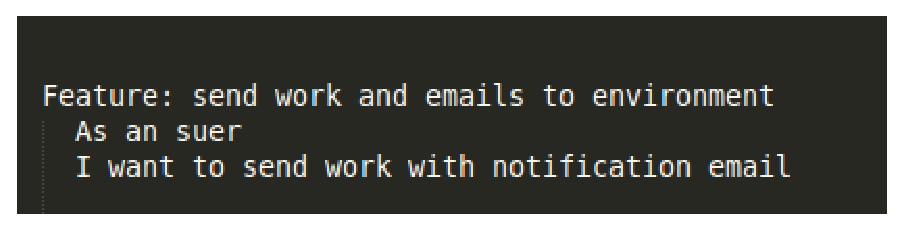
\includegraphics[keepaspectratio=true,scale=0.50]
      {figuras/noosfero_feature2.eps}
    \caption{Descrição do título (\textit{feature}) de um teste}
    \label{nosfero_feature}
\end{figure}

\item \textbf{Pré condições:} representado pela palavra-chave \textit{'background'}, define os passos 
precedem cada cenário de teste.

\begin{figure}[!h]
    \centering
    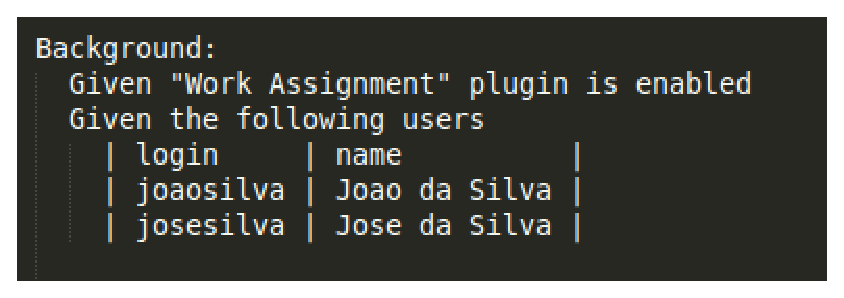
\includegraphics[keepaspectratio=true,scale=0.50]
      {figuras/noosfero_back.eps}
    \caption{Descrição de pré condições (\textit{background}) de um teste}
    \label{nosfero_feature}
\end{figure}

\item \textbf{Cenários:} representam parte concreta de como o software deve se 
comportar, e sendo a parte essencial do teste realizado no 
cucumber. Após a palavra-chave \textit{‘scenario’} define-se o nome do cenário em questão:
\item \textbf{Passos:} Cada cenario possui uma série de passos que demontram o seu 
comportamento, que são linhas simples iniciadas com as seguintes palavras-chaves: 
\textit{Given, When, Then, And, But}.
\item \textbf{Given:} Indica uma condição inicial para que o cenário seja executado, 
trata-se das pré-condições do cenário.
\item \textbf{When:} Indica o evento do cenário
\item \textbf{Then:} Indica o que é esperado após o evento ocorrer.

\begin{figure}[!h]
    \centering
    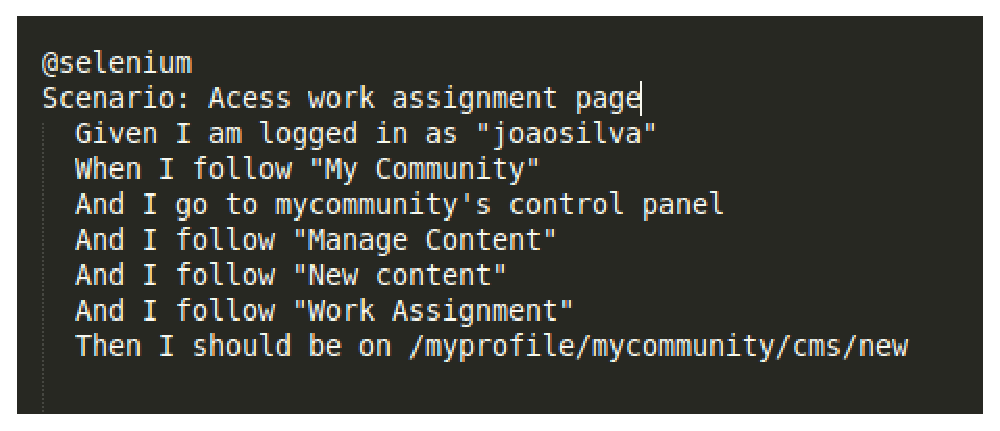
\includegraphics[keepaspectratio=true,scale=0.50]
      {figuras/noosfero_scenario.eps}
    \caption{Descrição do cenário (\textit{scenario}) de um teste}
    \label{nosfero_scenario}
\end{figure}

\end{enumerate}

Além do cucumber, também é utilizado um software chamado selenium, que é uma ferramenta
usada para desenvolver casos de testes a partir de \textit{web browsers}, como o mozilla firefox. Estas duas ferramentas, cucumber e selenium, utilizadas em conjunto, proporcionam ao desenvolvedor a facilidade ao escrever os casos de testes em linguagem pura simular a execução automática desses testes em um \textit{web browser}. Porém o cucumber não faz tudo em linguagem pura, é necessário que outro código seja desenvolvido, em Ruby, fazendo par por baixo dos panos com a linguagem pura e executando os testes~\cite{akita2011}.

\subsection{Testes Funcionais e Unitários}
%
Os testes funcionais tem como objetivo no desenvolvimento na plataforma noosfero, verificar a integração da aplicação desenvolvida. Os testes unitários são executados em conjunto com os testes funcionais, porém  com o objetivo de verificar trechos menores de códigos. Assim, os testes funcionais e unitários são escritos da seguinte forma:

\textbf{Setup:} indica as condições inciais dos testes, setando variáveis de ambiente e de configuração por exemplo.

\begin{figure}[!h]
    \centering
    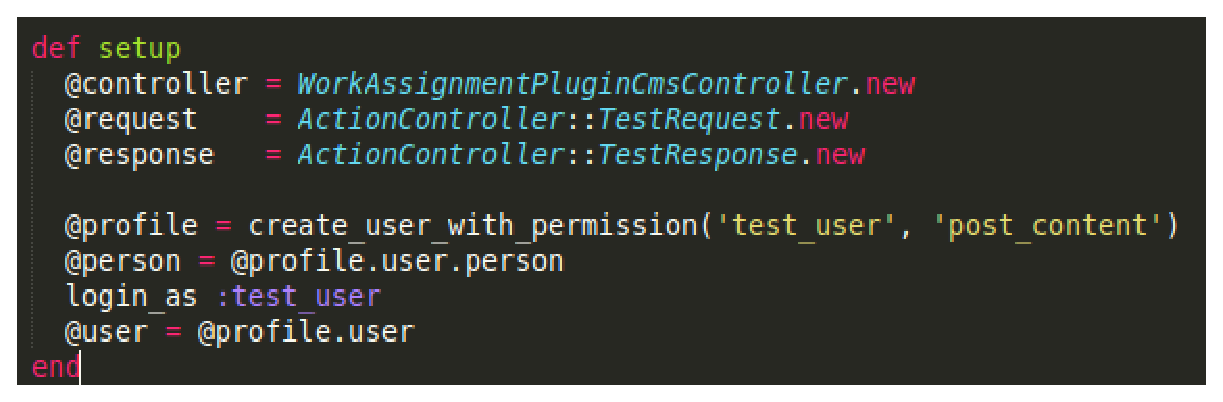
\includegraphics[keepaspectratio=true,scale=0.5]
      {figuras/teste_setup.eps}
    \caption{Descrição do setup de um teste}
    \label{nosfero_setup}
\end{figure}

\textbf{Título:} título do teste iniciado com a palavra \textit{‘should’} e finalizado com \textit{‘do’}

\textbf{Passos:} código que define o comportamento do teste

\textbf{Verificação:} Assertiva que verifica se a ação foi realizada como esperada.

\begin{figure}[!h]
    \centering
    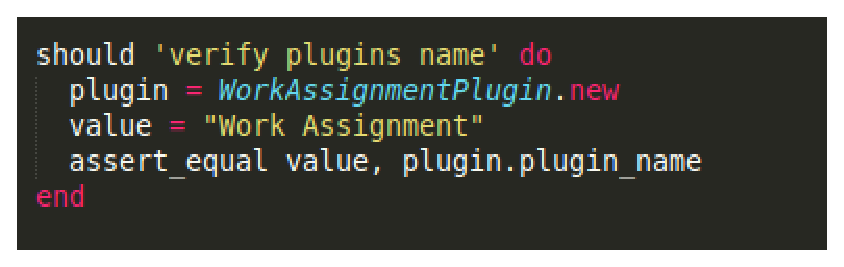
\includegraphics[keepaspectratio=true,scale=0.55]
      {figuras/teste_should.eps}
    \caption{Código de teste}
    \label{noosfero_should}
\end{figure}
%Done: alguns conceitos de testes têm referência e outros não.
%Done: colocar as referências
%Done: pontuar ao final da lista quais testes iremos tratar neste trabalho.

%------------------------------------------------------------------------------%
\section{Técnicas de desenvolvimento de testes automatizados}

Automação de testes é uma técnica voltada principalmente para a melhoria de 
qualidade dos sistemas de software. 
%
No processo de desenvolvimento de software é fundamental controlar o custo do 
processo de testes, para isso baterias de testes automatizados devem ser bem 
definidas e implementadas. Assim, é importante conhecer boas práticas e técnicas 
de desenvolvimento de testes automatizados.    
%
Existem várias técnicas de desenvolvimento de software com testes que influenciam 
diretamente na qualidade do sistema. Essas técnicas geralmente possuem um processo 
de atividades pequeno e simples, como TDD e BDD.

\subsection{TDD - Test Driven Development}

Desenvolvimento dirigido por testes, TDD \textit{(Test-Driven Develepment)}, 
é uma técnica de desenvolvimento de software que se dá pela repetição disciplinada 
de um ciclo curto de passos de implementação de testes e do sistema~\cite{koskela2007}.
%
O ciclo de TDD é definido pelos seguintes passos:
%
\begin{enumerate}
\item Implementar um caso de teste;
\item Implementar um trecho do código suficiente para o novo caso de teste ter sucesso 
de tal modo que não quebre os testes previamente escritos;
\item Se necessário, refatorar o código produzido para que ele fique mais organizado;
\end{enumerate}

\begin{figure}[h]
    \centering
    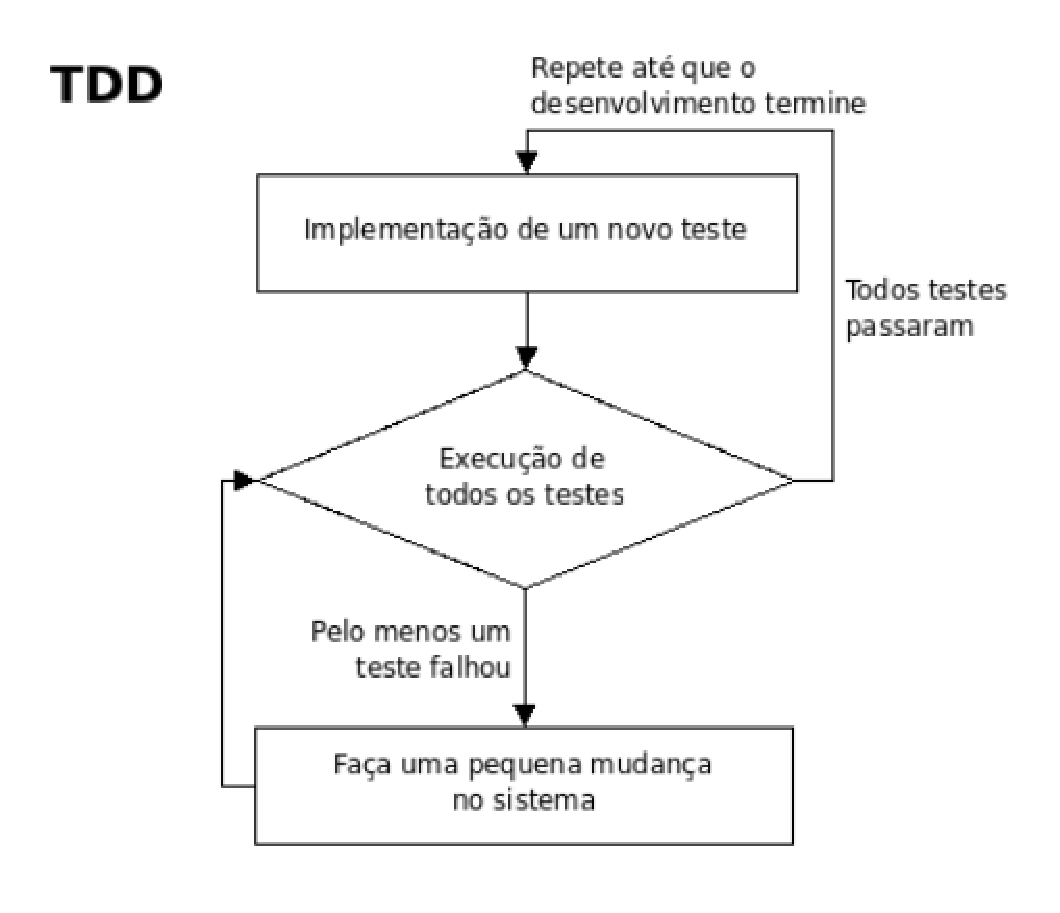
\includegraphics[keepaspectratio=true,scale=0.50]
      {figuras/tdd_ciclo.eps}
    \caption{Ciclo de atividades TDD~\cite{beck2002}}
    \label{tdd_ciclo}
\end{figure}

A técnica de desenvolvimento dirigido por testes foi definida no 
livro \textit{Test-Driven Development: By Example} por~\citeonline{beck2002}, como
representados na Figura~\ref{tdd_ciclo}.

Uma boa prática do TDD é a bateria de testes, que ajuda o desenvolvedor a evitar 
erros de regreção, quando o desenvolvimento de uma nova funcionalidade quebra uma 
já existente.
%
TDD também tende a contribuir com uma alta cobertura de código, uma 
fez que o desenvolvedor precisa escrever o testes antes da funcionalidade, 
possibilitando a criação de um código mais preciso, coeso e menos acoplado. 

Para ~\citeonline{massol2003}, o objetivo de TDD é código claro que 
funciona.
%
TDD propõe o desenvolvimento sempre em pequenos passo, deve-se escrever testes sempre 
para uma menor funcionalidade possível, escrever o código mais simples que faça o 
teste passar e fazer sempre apenas uma refatoração por vez~\cite{beck2002}. Assim o 
desenvolvedor se detém a criar soluções simples, sempre acompanhado de um constante 
\textit{feedback} dos testes.
%
O ciclo curto de passos definidos por TDD cria uma dependência forte entre codificação 
e testes, o que favorece e facilita a criação de sistemas com alta testabilidade~\cite{bernardo2011}. 
%
Índices altos de cobertura de código e testabilidade não garantem necessariamente 
qualidade do sistema, mas são métricas bem vistas para sistemas bem desenvolvidos.
%------------------------------------------------------------------------------%

\subsection{BDD - Behavior Driven Development}

Desenvolvimento dirido por comportamento \textit{(BDD - Behavior Driven Development)} 
é uma prática que recomenda o mesmo ciclo de desenvolvimento de TDD, contudo, induzindo 
a utilização de uma linguagem ubíqua entre cliente e equipe de desenvolvimento, subistituindo termos como assert, \textit{assert, test case, test suite} por termos 
mais comuns ao cliente, como \textit{should, context, specification}~\cite{bernardo2011}.

Embora seja principalmente uma ideia de como um processo de desenvolvimento de 
software deve ser gerenciado, a prática do BDD assume a utilização de ferramentas 
como suporte para o desenvolvimento de software~\cite{haring2011}. O BDD utiliza 
essas ferramentas para que os testes tenham como ponto de partida o compartamento 
das funcionalidade do sistema
%Done: confuso - "como ponto de partida o compartamento dos objetos"?

O BDD coloca em foco o comportamento em vez da estrutura de uma funcionalidade e faz isso em todos os níveis de desenvolvimento. Uma vez que nós reconhecemos isso, muda-se a forma como pensamos sobre desenvolvimento para fora do código. Assim começamos a pensar mais sobre as interações, sobre as pessoas e o sistema, do que sobre a 
estrutura do próprio sistema~\cite{chelimsky2010}.
%Done: em que contexto você está falando de objetos?

Para que o comportamento seja analisado, é necessário entender o ponto de vista do 
cliente/usuário, entendendo o comportamento que o sistema deve ter a partir da
visão do cliente/usuário. 
%
De acordo com ~\citeonline{chelimsky2010}, estes são os três príncipios do BDD:

\begin{enumerate}
\item \textbf{O suficiente é suficiente:} parte da ideia de gerenciar o esfoço no 
planejamento inicial do sistema, para não fazer menos nem mais do que o necessário 
para começar, o que se aplica também ao processo de automação.

\item \textbf{Agregar valor às partes interessadas:} Se você está fazendo algo que 
não agrega valor ou que não aumenta a capacidade de agregar valor, pare e faça outra 
coisa em seu lugar.

\item \textbf{Tudo é comportamento:} Do código à aplicação, pode-se usar o mesmo 
pensamento e as mesmas construções linguísticas para descrever o comportamento, em 
qualquer nível de granularidade. 
\end{enumerate}
%Done: parte da lista está referenciada e outra parte não...

O comportamento do sistema é descrito em histórias de usuário, que são 
escritas com a participação tanto de clientes como desemvolvedores do sistema. Assim 
cada história de usuário deve seguir, de certa forma, a seguinte estrutura:
%Done: com não explicaram métodos ágeis de forma mais didática e prática, aqui o leitor não sabe o que é um histório de usuário...

\textbf{Título:} do que se trata a história.

\textbf{Narrativa:} deve identificar as partes interessadas para essa história, as 
funcionalidades requeridas, e o benefício deste comportamento. A narrativa de uma 
história pode ter vários formatos.

\textbf{Critério de aceitação:} descrição de cada caso específico da narrativa, 
iniciado pela especificação da condição inicial do cenário, seguidos pelos estados 
que ativam este cenário, finalizado pelos estados esperados ao final do cenário.


\subsection{Considerações Finais}

Testes automatizados devem ser desenvolvidos com prioridade, buscando um rápido 
\textit{feedback}, contribuindo assim com a melhoria do sistema. Para isso é 
necessário que os cenários de testes estejam bem definidos junto à equipe.

No próximo capítulo abordaremos um estudo sobre usabilidade e como esta área é inserida no processo de desenvolvimento empírico.

%Done: até fez uma conclusão, mas não fez o link com o que vem pela frente.
